\chapter{Transaction Scheduler}
\label{scheduler}

A scheduler is responsible for executing transactions according to the fairness criteria set forth in Chapter~\ref{model}.
Of particular interest is the design and implementation of general-purpose schedulers that are capable of executing transactions in parallel.
The main inputs to a scheduler are the transactions enumerated by the composition analysis.
The access sets calculated for each transaction are used by concurrent schedulers to avoid non-deterministic state transitions.
In this chapter, we introduce some of the issues involved in designing and implementing a scheduler for reactive components, through a series of increasingly complex scheduler designs.
The two concrete implementations described later will draw upon the designs of these schedulers.

\section{The Transaction Scheduling Problem}
\label{scheduling_problem}

A scheduler is responsible for mapping transactions to processor cores so that they can be executed according to the semantics of reactive components.
As described in Chapter~\ref{model}, concurrent execution is modeled by a scheduler that serially and repeatedly executes atomic transactions according to fairness, which means that all enabled transaction must eventually be executed.
A scheduler implementation supporting concurrent execution must take care to preserve the fairness and atomicity required by the model.
A scheduler is \emph{fair} if it executes each transaction an infinite number of times or terminates by reaching a fixed point.
A scheduler is \emph{safe} if it avoids conditions where one transaction is changing the state of a component while another transaction is reading or writing the same state.
The execution of a transaction in a safe scheduler is logically atomic.

A scheduler is \emph{responsible} if it only terminates when a fixed point has been reached.
Termination is not a requirement for a scheduler, but it is useful from the perspective of testing and evaluation.
We are interested in designing fair, safe, and responsible schedulers, as these schedulers enforce the semantics of reactive components.

We model a scheduler as a state transition system consisting of a set of possible states $S$, an initial state $s_0 \in S$, and a transition function $\sigma: S \to S$.
The function $\sigma$ is applied to the current scheduler state $s$ to generate the next scheduler state $s' = \sigma (s)$.
To refer to previous scheduler states, we assign a logical time $t \in \mathcal{N}$ to each scheduler state so that $s(t + 1) = \sigma (s(t))$.
Using this notation, the initial state of the scheduler is $s(0) = s_0$.
The definitions of $S$, $s_0$, and $\sigma$ will be unique to each scheduling algorithm.
We are interested in the properties of $\sigma$ as they relate to enforcing the scheduling semantics of reactive components and how these properties help or hinder a scheduler implementation.

The generic state of a scheduler is modeled as a vector where each element of the vector contains the scheduling state associated with a particular transaction.
Let $s \in S$ be a generic scheduler state and let $T$ be the set of transactions.
The value $s_u(t)$ represents the scheduler state for transaction $u \in T$ at time $t$.
Each value $s_u(t)$ is a pair $(p, q)$.
The value $p \in \{\bot, 0, 1\}$ represents the precondition of the transaction known by the scheduler as either unknown ($\bot$), false (0), or true (1).
The value $q \in Q = \{\mathit{Idle}, \mathit{Eval}, \mathit{Exec}\}$ represents the state of the transaction as either being idle, evaluating the precondition, or executing the immutable and then mutable phases.
Initially, all transactions start with an unknown precondition in the idle state:
\begin{equation}
  \forall u \in T : s_u(0) = (\bot, \mathit{Idle})
\end{equation}

In the model, the precondition of each transaction is always defined and known since the state against which the preconditions are evaluated is always defined and known due to atomicity.
In a real scheduler, the execution of a transaction takes time and the state of all involved components is not defined for this duration.
Consequently, the values of preconditions derived from this state are also not defined during the same duration.
After a transaction, all preconditions based on any mutated state are undefined and must be re-evaluated to determine if they are true or false.

\begin{figure}
\centering
%\resizebox{\textwidth}{!}{%
\begingroup
\fontsize{10pt}{12pt}\selectfont
\begin{tikzpicture}
  [->,-triangle 60, node distance=3cm, auto, every loop/.append style={-triangle 60}]

  \node[initial,state] (I)              {$I$};
  \node[state]         (V) [above of=I] {$V$};
  \node[state]         (X) [right of=I] {$X$};

  \path (I) edge [bend left] node {$a$} (V)
            edge [bend left] node {$e$} (X)
        (V) edge [bend left] node {$d$} (I)
            edge             node {$b$} (X)
        (X) edge [bend left] node {$c$} (I);

  \path (I) edge [loop below] node {$\lambda$} ();
  \path (V) edge [loop above] node {$\lambda$} ();
  \path (X) edge [loop right] node {$\lambda$} ();

\end{tikzpicture}
\endgroup
%}%
\caption{State transition diagram for the state component of the dynamic transaction state.
  $I$ represents $\mathit{Idle}$, $V$ represents $\mathit{Eval}$, and $X$ represents $\mathit{Exec}$.
  \label{dt_state}}
\end{figure}

The dynamic transaction state $s_u(t)$ is itself a state transition system and much of the challenge in designing a scheduler revolves around the details of enforcing this transition system for concurrently executing transactions.
Figure~\ref{dt_state} shows the state transition diagram for the state component of the dynamic transaction state ($q$ of $s_u(t)$).
Each state has a self loop that allows a transaction to stay in the same state while another transaction changes state (indicated by $\lambda$).
There are two main paths through the transition system.
The path $abc$ corresponds to evaluating the precondition and immediately executing the immutable and mutable phases.
The path $adec$, for example, corresponds to evaluating the precondition and later executing the immutable and mutable phases.
Let $\Gamma$ be the set of transitions indicated in Figure~\ref{dt_state}.
Each element $\gamma \in \Gamma$ is a pair in $Q \times Q$.
The following condition states that every transition in a scheduler must obey the transition system described in Figure~\ref{dt_state}:
\begin{equation}
  \forall t, u : (s_u(t).q, s_u(t+1).q) \in \Gamma
\end{equation}
The precondition of a transaction is established as true or false as a result of leaving the $\mathit{Eval}$ state (transitions $b$ and $d$ in figure~\ref{dt_state}):
\begin{equation}
  \label{pre_establish}
  \forall t, u, s_u(t).q = \mathit{Eval} \land s_u(t+1).q \neq \mathit{Eval} : s_u(t+1).p \in \{0,1\}
\end{equation}
The precondition of a transaction must be true while executing the immutable and mutable phases:
\begin{equation}
  \label{pre_true}
  \forall t, u : s_u(t).q = \mathit{Exec} \implies s_u(t).p = 1
\end{equation}

A transaction that mutates the state of one or more components invalidates the precondition of all transactions whose preconditions are derived from the same state.
Let $\mathit{pre}: T \to H$ be a function that maps a transaction to the set of access pairs corresponding to the precondition of a transaction.
Let $\mathit{imm}(u)$ and $\mathit{mut}(u)$ be similarly defined functions that return the immutable phase access set and mutable phase access set for transaction $u \in T$.
All of these functions may be computed as part of composition analysis.
The set of transactions that are potentially affected by a given transaction $u \in T$ is given by the following function:
\begin{equation}
  \label{affected}
  \mathit{affected}(u) = { v \in T : \mathit{race}(\mathit{mut}(u), \mathit{pre}(v)) }
\end{equation}
The result of a transaction being executed has the effect of invalidating the precondition for all affected transactions:
\begin{multline}
  \forall t, u : s_u(t).q = \mathit{Exec} \land s_u(t+1).q \neq \mathit{Exec} \implies \\ \forall v \in \mathit{affected}(u) : s_v(t+1).p = \bot
\end{multline}
The previous requirement represents a worst case scenario where the transaction mutates all components in the mutable access set.
An obvious optimization is to only invalidate preconditions derived from the subset of instances that actually changed state.

A scheduler is safe if it avoids data races among the set of active transactions.
We define the dynamic access set of a transaction as follows:
\begin{equation}
  \label{access}
  \mathit{access}(s_u) = \begin{cases}
    \emptyset & \text{if $s_u.q = \mathit{Idle}$} \\
    \mathit{pre}(u) & \text{if $s_u.q = \mathit{Eval}$} \\
    \mathit{imm}(u) \cup \mathit{mut}(u) & \text{if $s_u.q = \mathit{Exec}$}
    \end{cases}
\end{equation}
A scheduler state is safe if there are no data races:
\begin{equation}
  \mathit{safe}(s) = \forall u, v \in T, u \neq v : \lnot \mathit{race} (\mathit{access}(s_u), \mathit{access}(s_v))
\end{equation}
A scheduler is safe if it only enters safe states:
\begin{equation}
  \label{race}
  \forall t : \mathit{safe}(s(t))
\end{equation}

%% The safety requirement expressed in Equation~\ref{race} influences every voluntary scheduling decision.
%% Consider the set of possible next states for a scheduler.
%% The transitions in figure~\ref{dt_state} can be classified into two groups.
%% Transitions $a$, $b$, and $e$ are voluntary and result in non-empty access sets while $d$ and $c$ are involuntary and result in empty access sets (Equation~\ref{access}).
%% Thus, we limit the discussion to scheduling steps where the scheduler is making a voluntary transition.
%% Let $\mathit{vol}(t) \subseteq T$ represent the subset of transactions that are candidates for a voluntary transition at time $t$ and let $\mathit{next}(u)$ represent the next transition state according to the system of figure~\ref{dt_state}.
%% Also, let $s(t) \downarrow u$ represent the result of substituting transaction state $u$ into $s(t)$.
%% A set of possible next states is given by:
%% \begin{equation}
%%   \mathit{candidates}(t) = \bigcup_{u \in \mathit{vol}(t)} s(t) \downarrow \mathit{next}(u)
%% \end{equation}
%% However, not every state in $\mathit{next}(t)$ is a valid state due to Equation~\ref{race}.
%% A refined set of next states is then:
%% \begin{equation}
%%   \mathit{next}(t) = \{ s \in candidates(t) : safe(s) \}
%% \end{equation}

In a fair scheduler, an enabled transaction cannot be postponed indefinitely.
Argument by contradiction is one approach to demonstrating that a scheduling algorithm is fair.
If one assumes that a scheduler is not fair, then there must be some scheduler state $s(t_c)$ that contains a transaction $u$ that is enabled in every subsequent state but never executed.
The ``enabledness'' described in the previous sentence is not the value $p$ in the definition of $s_u(t)$ which is the value known by the scheduler.
Rather, it refers to the actual value of the precondition based on the state contained in the component instance.
The argument is completed by demonstrating that the scheduler does in fact execute $u$.
For example, a scheduler that processes transactions in first-in first-out (FIFO) order eventually executes every transaction in the queue.

A scheduler design must reconcile the forces arising from the basic execution model, fairness, safety, and efficiency.
The basic execution model forces the scheduler to establish preconditions (Equation~\ref{pre_establish}) before executing the immutable and mutable phases (Equation~\ref{pre_true}).
Fairness compels the scheduler to execute certain transactions while safety compels the scheduler to avoid executing certain transactions (Equation~\ref{race}).
With respect to efficiency, a scheduler design may attempt to exploit the concurrency available in the set of transactions through parallel execution.

To illustrate the interplay among these forces, consider a concurrent and work-conserving scheduler.
Let the system consist of the set of transactions $S \cup \{ \tau \}$ where $S$ is a set of transactions that are safe with respect to each other and $\tau$ is a transaction that is not safe with respect to all transactions in $S$.
Thus, at any given time, the scheduler can be executing transactions in $S$ or $\tau$.
Suppose the scheduler is concurrently executing two transactions from $S$.
When one of the transactions terminates, the scheduler must immediately execute another transaction since it is work conserving.
For safety, the scheduler will execute another transaction from $S$ as it is unsafe to execute $\tau$.
This pattern of behavior induced by the work conserving nature of the scheduler may perpetually deny service to $\tau$.
For fairness, the scheduler must refrain from executing another transaction so that the $\tau$ transaction can be serviced.
Thus, with respect to parallel and concurrent execution, a scheduler design must balance gains in performance from exploiting parallelism with the requirement of fairness.

The scheduling problem for reactive components, then, is:  given a set of active transactions, select the next transaction for evaluation (precondition) or execution (immutable and mutable phase) subject to fairness and safety.

\section{Scheduler Classes}

Different factors may influence the design of transaction schedulers, which we distinguish according to four dimensions.
A given scheduler may be:  \emph{lazy} or \emph{eager}, \emph{oblivious} or \emph{knowledgeable}, \emph{cautious} or \emph{speculative}, and \emph{non-preemptive} or \emph{preemptive}.

\paragraph{Lazy and eager schedulers.}
A scheduler may be \emph{lazy} or \emph{eager} with respect to evaluating preconditions.
A lazy scheduler defers evaluating the precondition until the transaction is selected for execution (path $abc$ in Figure~\ref{dt_state}).
An eager scheduler evaluates preconditions after the state upon which they are based changes (path $ad$ in Figure~\ref{dt_state}).
The perceived benefit of a lazy scheduler is that it may reduce overhead by not evaluating preconditions while the perceived benefit of an eager scheduler is that it may only select actions which are enabled, which may result in more efficient use of acquired resources.

\paragraph{Oblivious and knowledgeable schedulers.}
We have considered two kinds of schedulers with respect to safety.
The first is an \emph{oblivious} scheduler that doesn't have direct access to the (global) scheduler state and therefore can't know the set of next states.
An oblivious scheduler selects a transaction and then determines if the transaction is safe to execute.
This typically involves a locking mechanism to ensure that all of the instances in the requisite access sets are available.
The second kind of scheduler is a \emph{knowledgeable} scheduler that does know the global scheduler state.
A knowledgeable scheduler can be proactive and maintain a set of transactions that are safe with respect to the set of active transactions.
This would allow a knowledgeable scheduler to efficiently select a safe action.
The open question is whether or not the efficiency of selection overcomes the overhead of maintaining the set of safe transactions.

\paragraph{Cautious and speculative schedulers.}
A \emph{cautious} scheduler avoids all race conditions and always satisfies the safety requirement of Equation~\ref{race}.
A \emph{speculative} scheduler optimistically evaluates preconditions and executes transactions but aborts them if a conflict is discovered.
Transactional memory is one technology that could be used to build a speculative scheduler.
For this work, we will assume that preconditions, immutable phases, and mutable phases are not aborted and leave the application of transactional memory to reactive components as future work.

\paragraph{Non-preemptive and preemptive schedulers.}
An \emph{active} transaction is one whose precondition is being evaluated or whose immutable or mutable phase is being executed.
An active transaction need not physically occupy a processor core.
This condition occurs in \emph{preemptive} schedulers that can interrupt a precondition, immutable phase, or mutable phase to do other work.
In contrast, a \emph{non-preemptive} scheduler does not interrupt the execution of a transaction, i.e., transactions are physically atomic.
Preemption may be useful to reduce the latency of transactions, support real-time priorities, etc.
We leave the application of preemption to reactive component schedulers as future work.

\section{Scheduler Design}

The previous sub-section illustrated a number of design dimensions for reactive component schedulers:  lazy vs. eager, oblivious vs. knowledgeable, cautious vs. speculative, and non-preemptive vs. preemptive.
For tractability, we will focus on the design and implementation of particular schedulers that are lazy, oblivious, cautious, and non-preemptive, and leave a more complete exploration of the design space for future work.
The goal of the following discussion is to introduce some of the issues when designing and implementing a scheduler, through a series of increasingly complex scheduler designs.
We will describe the concurrent schedulers in terms of \emph{threads}, which may be dedicated to physical processor cores or scheduled on one or more cores by an operating system.

%% \paragraph{Scheduler criteria.}
%% A scheduler is \emph{fair} if it meets the fairness criteria set forth in Chapter~\ref{model}.
%% A scheduler is \emph{safe} if it avoids conditions where one transaction is changing the state of the component while another transaction is reading or writing the same state.
%% A scheduler is \emph{responsible} if it only terminates when the precondition for every action is false.
%% Obviously, we are interested in fair, safe, and responsible schedulers as these schedulers enforce the semantics of reactive components.
%% The final criteria for a scheduler is efficiency which typically refers to either the computational complexity or storage complexity associated with its operation.
%% % Of primary interest is the \emph{selection efficiency} or the amount of computation required for the scheduler to determine the next action to execute.

\paragraph{Serial round-robin scheduler.}
Perhaps the simplest scheduler that can be implemented is a serial round-robin scheduler.
This design may be appropriate in the context of uniprocessor embedded systems with tight resource constraints.
The scheduler repeatedly cycles through the list of transactions, evaluating the precondition of each transaction and executing the immutable and mutable phases if the precondition was true.
If no transaction is executed in a cycle, then the scheduler terminates.
This scheduling algorithm is fair by virtue of the strict round-robin policy, safe from the fact that it is serial and non-preemptive, and responsible by definition.
The \emph{selection efficiency} of a scheduler is the number of transactions that must be selected before executing an enabled transaction or terminating.
The selection efficiency of this algorithm is $O(|T|)$ as illustrated by a system where one transaction that is perpetually enabled while all of the other transactions are perpetually disabled.

\paragraph{Serial scheduler with a transaction work queue.}
The perceived weakness of the serial round-robin scheduler is the overhead of evaluating preconditions that evaluate to false.
So, instead of cycling through the list of transactions, this scheduler maintains a work queue of transactions whose preconditions are true.
At initialization time, the scheduler populates the queue by evaluating the precondition of each transaction in the system.
The scheduler then repeatedly takes a transaction from the queue, executes it, and then inserts any newly enabled transactions, making this scheduler an eager scheduler.
To find newly enabled transactions, the scheduler uses the access set generated during composition analysis.
That is, after executing a transaction, the scheduler tests all of the transactions for the components in the access set and adds them to the queue if necessary.
Alternatively, the scheduler may assume that the precondition is true and insert the transaction, knowing that the precondition will be re-evaluated when the transaction is selected.
The scheduler terminates when the work queue is empty.
This scheduling algorithm is fair if the work queue is processed in first-in first-out (FIFO) order, safe because the algorithm is serial and non-preemptive, and responsible since an empty work queue implies no transaction is enabled.

The pathological scenario for the serial round-robin scheduler applies to this scheduler as well, so the worst-case selection efficiency of the algorithm is $O(|T|)$.
Assume that the most complex transaction in the system involves $c$ components and some component has a system-wide maximum transaction count of $a$.
In the worst case, the scheduler must evaluate $c \times a$ preconditions for every transaction that it executes.
Thus, the overhead associated with this scheduler is related to the compositional structure of the system that it is executing.
This overhead may be acceptable for systems where $c$ and $a$ are small or for systems whose average work queue size is small compared to the total number of transactions in the system.
This suggests that the average number of enabled transactions compared to the total number of transactions may be a useful way to analyze reactive component systems and schedulers.
For example, the serial round-robin scheduler would be appropriate for a \emph{heavily enabled} system while the serial scheduler with a transaction work queue would be appropriate for a \emph{lightly enabled} system.

\paragraph{Serial scheduler with an instance work queue.}
This scheduling algorithm attempts to squeeze a little more performance from the single-threaded scheduler with a transaction work queue.
The significant difference is that after the scheduler executes a transaction, it places the component instances that might have changed state into the work queue.
The work queue is initialized with all of the components in the system.
When processing a component on the work queue, the scheduler cycles through all of the transactions for that particular component.
The potential increase in performance comes from deferring the evaluations of the preconditions until absolutely necessary, i.e., lazy scheduling.
The scenario on which this scheduler attempts to capitalize is when some components are rarely involved in transactions.
An instance is enabled if at least one of its transactions is enabled.
Thus, this scheduler is appropriate for systems that are lightly enabled from the instance perspective.

\paragraph{Concurrent global round-robin scheduler.}
This scheduler runs $P > 1$ copies of a round-robin scheduler in parallel.
To be safe, we must devise a protocol that allows the threads to avoid concurrently executing transactions that may mutate the same state.
Using the assumption that a component instance is a proxy for its state variables, the scheduler locks all instances in the access set before evaluating the precondition and executing the transaction.
Recall that composition analysis determines the set of components that are involved in a transaction and how they are accessed ($\mathit{Read}$ or $\mathit{Write}$).
The acquired lock corresponds to the access type, which allows multiple threads to be reading a component but only one thread to be writing.
The locks are acquired in a determined order to avoid deadlock (Havender's Principle).
The concurrent global round-robin scheduler is fair so long as the underlying locking mechanism is fair, i.e., there is no reader or writer starvation.
The algorithm is also responsible, as each thread proves to itself that there are no enabled transactions left in the system.

An important concern with this algorithm is the locking required to coordinate access to component instances.
One negative characteristic caused by the locking is that a thread may become idle while waiting for a lock.
Thus, we might look for alternatives that allow a thread to do other useful work while waiting for a lock.
Another goal might be to look for ways to coordinate access to component instances without using locks at all.
Some of these ideas are explored later in this chapter.

\paragraph{Concurrent partitioned round-robin scheduler.}
Rather than have each thread cycle through the entire list of transactions, the concurrent partitioned round-robin scheduler divides the list of transactions among the available threads.
Like the global version, this algorithm is fair if the underlying locking mechanism is fair.
Similarly, this algorithm is safe as locks are used to coordinate access to component state.
However, for this algorithm to be responsible, we must add a protocol that allows the threads to detect that the system has reached the termination condition.

The termination protocol consists of a barrier synchronization and then a check to establish the termination condition.
The termination protocol begins when a scheduler thread sends a termination request to the \emph{manager thread}.
To process a termination request, the manager thread stops each scheduler thread and then checks that all transactions are disabled.
If all of the transactions are disabled, the system terminates.
Otherwise, the manager thread restarts the scheduler threads.
A scheduler thread may choose to request termination at any time and different heuristics may be used to determine when a scheduler thread makes the termination request.
Deferring the request has the advantage of avoiding the termination protocol overhead.
For example, a scheduler thread might wait until it makes a complete pass through its list of transactions without executing one before making the request.

Such a centralized termination protocol is rather disruptive as it must stop the system to check for termination.
Thus, one goal may be to let a thread idle itself and be woken up by active neighbors.
Similarly, the scheduler threads can check for the termination condition in parallel and wake up all of their neighbors if a transaction is enabled.
Finally, the manager thread may be done away with entirely and the protocol rewritten as a distributed protocol, as we discuss below.

\section{Scheduler Implementations}

We now describe two specific scheduler designs that we chose for implementation and evaluation.
Each scheduler takes a different approach to the design dimensions described previously, resulting in distinct consequences for systems that use it.

\paragraph{Concurrent scheduler with a global instance work queue.}
The first scheduler that we implemented was a concurrent scheduler with a global instance work queue.
The work queue is initialized to contain all of the instances in the system.
The scheduler threads take an instance from the work queue, select and execute all transactions in the instance, and insert any instances that might have changed state back into the work queue.
Fairness is achieved by processing the queue in FIFO order and safety is achieved through the aforementioned locking scheme.
The termination protocol for this scheduler involves counting the number of instances that are currently in the queue and the number of instances currently being processed by the scheduler threads.
When this count drops to zero, there are no enabled instances in the system and the system may terminate responsibly.

One potential weakness of this scheduler is the synchronization required to coordinate access to the work queue, which adds a communication overhead and may create contention if the scheduler threads are lightly loaded, i.e., they frequently return to the queue looking for work.
Thus, the scalability of this scheduler is a concern.

\paragraph{Concurrent partitioned round-robin scheduler with asynchronous locking and distributed termination.}
One of the goals when designing this scheduler was to avoid the blocking behavior and overhead of locking observed during out evaluations of the concurrent scheduler with a global instance work queue.
The pthreads reader/writer locks used to protect each component instance were replaced by asynchronous reader/writer locks implemented in user-space.
The asynchronous locks consist of a spin lock, variables indicating the status of the lock, and a queue of requests.
To acquire a lock for a component, a scheduler thread first acquires the spin lock and then checks if the lock can be acquired immediately, which it can if either the lock has no owner or the thread is a reader (i.e., it is requesting a read lock); the lock has already been locked by another reader; and there are no writers in the queue.
Otherwise, the request is placed on the queue.
A scheduler thread failing to acquire the lock can either idle or attempt to execute a different transaction.
When a lock is unlocked, the thread at the front of the queue is notified so it may resume processing the transaction that it was attempting to execute.
The protocol avoids reader and writer starvation and ensures fairness since the queue is processed in FIFO order.
This scheduler is \emph{work conserving} since a scheduler thread continues to execute transactions instead of blocking.
However, scheduler threads do not steal work from other threads.

The aforementioned centralized termination protocol has the potential to be disruptive.
Thus, the motivation for a distributed termination protocol is to keep the scheduler threads as busy as possible meaning that the termination protocol is started infrequently and the termination protocol itself aborts as early as possible if the termination condition has not been reached.
For this scheduler, the threads are arranged in a ring and communicate using asynchronous message queues.
Messages are stamped with the id of the originating thread.
The protocol forwards messages around the ring so a thread receiving a message from itself knows that all of the threads have processed that message.

Like the centralized version, the ring-based distributed termination protocol consists of a synchronization phase and checking phase.
Scheduler threads begin in the RUN state where they are actively cycling through their lists of transactions.
When a scheduler thread determines that termination may be possible, it sends a message to its neighbor indicating that it is entering the SYNC state.
If the neighbor thread is in the RUN state, it resolves to send a reset message the next time it executes a transaction which means that the termination condition has not been established.
Otherwise, the neighbor thread itself is already in the SYNC state and forwards the message.
Reset messages are unconditionally forwarded around the ring and cause all threads to enter the RUN state.
Synchronization messages are only forwarded if the thread receiving the message is in the SYNC state.
Thus, if a thread receives its own synchronization message, all other threads in the scheduler are in the SYNC state.
Multiple threads may receive their own synchronization message at the same time.

The goal of the synchronization phase is to establish a common point of reference for determining if any transaction is enabled.
When a thread receives its own synchronization message, it sends a message to its neighbor that it is entering the CHECK state.
This message is forwarded around the ring causing all of the threads to enter the CHECK state.
The CHECK state is like the modified RUN state in that any executed transaction causes a reset message to circulate around the ring.
A thread that cycles through its list of transactions and finds no enabled transactions sends a wait message to its neighbor and enters the WAIT state.
If the neighbor is in the WAIT state, it forwards the message.
If a thread receives its own wait message, then all of the threads are in the WAIT state and the termination condition has been established.
Upon receiving its own wait message, a thread sends a termination message causing all threads to terminate.

\section{Scheduler Evaluation}

The utility of the reactive component model rests on the ability to execute reactive programs effectively.
The challenge, then, is to design and implement effective schedulers subject to the constraints and limitations imposed by the model.
The exercise of developing and evaluating schedulers may suggest possible improvements to the model or provide evidence that core features of the model resist efficient implementation.
The definition of an effective scheduler will vary by platform and problem domain.
For example, embedded systems may prefer a single-threaded scheduler with minimal memory requirements and power-awareness.
Our focus in this work is to make progress on general-purpose concurrent schedulers.
We propose the following metrics for the evaluation of a general-purpose scheduler:
\begin{description}
\item[Throughput:] the number of transactions executed per second.
Given the same system, a scheduler with higher throughput is preferable to a system with lower throughput as it is accomplishing more work per unit of time.
Throughput can also be defined for specific problems by defining a unit of work and measuring the number of work units processed per unit of time.
\item[Latency:] the amount of time between an transaction becoming enabled and being executed.
The goal in measuring the latency between a transaction becoming enabled and its execution is to quantify the responsiveness of the scheduler.
An interactive application may prefer a scheduler that executes enabled transactions promptly to aid in providing a good user experience or other benefit.
Like throughput, latency may also be defined for units of work.
\item[Utilization:] the fraction of the CPUs used.
Utilization is a measure of how efficiently the scheduler is using the CPUs and can be used to quantify an improvement in throughput or latency.
For example, a 10\% increase in throughput accompanied by a 10\% increase in utilization may be acceptable while a 10\% increase in throughput with a 100\% increase in utilization may not be acceptable.
\end{description}
Both throughput and latency may be considered for individual transactions, or may be aggregated over all transactions in the system.

\paragraph{Evaluation approach.}
We used two variants of the clock system from Chapter~\ref{model} to evaluate the two scheduler implementations.
The first variant is the fully-factored clock system augmented with counters that cause termination\footnote{https://github.com/jrw972/rc/blob/master/samples/clock3.rc}.
In this system, there are three components of interest:  the Client, the Server, and the Counter.
This system has three transactions:
\begin{itemize}
  \item Request - The client requests the time from the server.  This involves the Client and the Server.
  \item Response - The server responds with the time.  This involves the Client, the Server, and the Counter.
  \item Tick - The counter increments the current time.  This involves the Counter.
\end{itemize}
This system will be denoted as the \emph{AsyncClock} system.

\begin{figure}
\centering
\resizebox{.5\textwidth}{!}{%
\begingroup
\fontsize{10pt}{12pt}\selectfont
\begin{tikzpicture}

\node[draw, ellipse] (Request) at (0,0) {Request};
\node[draw, ellipse] (Response) at (3,0) {Response};
\node[draw, ellipse] (Tick) at (1.5,-1) {Tick};

\draw (Request) -- (Response);
\draw (Tick) -- (Response);

\end{tikzpicture}
\endgroup
}%
\caption{Race graph for the AsyncClock system.  Each node is a transaction.  Nodes sharing an edge cannot be executed concurrently due to potentially mutated shared state. \label{clock_system_mutex}}
\end{figure}

Figure~\ref{clock_system_mutex} shows a \emph{race graph} for the AsyncClock system.
Each node in the graph is a transaction $u \in T$.
Let $\mathit{acc}(u) = \mathit{pre}(u) \cup \mathit{imm}(u) \cup \mathit{mut}(u)$.
An edges exists between two nodes $u,v \in T$ if $\mathit{race}(\mathit{acc}(u), \mathit{acc}(v))$.
Nodes sharing an edge cannot be executed concurrently due to potentially mutated shared state.
Conversely, nodes that are not linked by an edge can be executed concurrently.
For the purpose of evaluating schedulers, the clock system has the important characteristic that Request and Tick can be executed concurrently while Response must be executed independently.
Another useful feature of this system is that each component has exactly one transaction, and thus, a  work queue of instances may also be viewed as a work queue of transactions.

The second variant is a simplified version of the clock system consisting of a Tick transaction that increments the counter and a Request transaction that uses a getter to sample the counter\footnote{https://github.com/jrw972/rc/blob/master/samples/clock4.rc}.
The counter creates a race between the two transactions so that they cannot be executed concurrently.
This system will be denoted as the \emph{SyncClock} system.

For comparison, we implemented threaded versions of the AsyncClock and SyncClock systems using the POSIX threads library (pthreads).
The AsyncClock implementation attempts to preserve the spirit of the AsyncClock system by being as asynchronous as possible.
This implementation uses three threads corresponding to the Request, Response, and Tick transactions.
The Request and Response threads share a flag variable that is protected by a mutex and condition variable, to implement the asynchronous request/response protocol.
The Response and Tick threads share a counter variable that is protected by a mutex.
The SyncClock implementation attempts to preserve the spirit of the SyncClock system.
In this design, there is one thread sampling the counter while another thread is incrementing the counter.
The two threads synchronize access to the counter through a single mutex.
For convenience, experiments involving a pthreads implementation will be labeled \emph{Thread}, experiments involving the concurrent scheduler with a global instance work queue will be labeled \emph{Instance}, and experiments involving the concurrent partitioned  round-robin scheduler with asynchronous locking and distributed termination will be labeled \emph{Partitioned}.

The AsyncClock and SyncClock systems were executed 1,000 times to profile the performance of each scheduler.
The programs are instrumented with profiling code that records the total execution time and timestamps for each transaction.
The timestamps are stored in memory and written after the scheduler terminates to avoid disruptions in timing due to output.
The Request and Tick transactions were limited to 10,000 executions.
Thus, each SyncClock run generates 20,000 data points.
In the AsyncClock system, the relationship between Request and Response causes Response to be executed 10,000 times as well.
Thus, each AsyncClock run generates 30,000 data points.
The throughput for a single run is determined by dividing the total number of transactions (20,000 or 30,000) by the total time used for execution.
The utilization was determined using the \verb+time+ utility and the number of context switches was determined using the \verb+getrusage+ system call before and after the execution of the system.
The latency for each transaction is determined by computing the difference between the transaction start time and the end time of the enabling transaction.
For the SyncClock system, this is $Request_{t+1} - Request_{t}$ and $Tick_{t+1} - Tick_{t}$.
For the AsyncClock system, this is $Request_{t+1} - Response_{t}$, $Response_{t+1} - Request_{t}$, and $Tick_{t+1} - Tick_{t}$.
For the SyncClock system, $1,000 \times 20,000 = 20,000,000$ latency points were collected.
For the AsyncClock system, $1,000 \times 30,000 = 30,000,000$ latency points were collected.

Placing all transactions in a run on a timeline according to their start times, we define the \emph{entanglement} of a run to be the number of adjacent transactions on the timeline that were executed in different threads.
The entanglement is used to measure the granularity of the concurrency between the scheduler threads.
Given that each run executes the same number of transactions, a high entanglement indicates ``fine'' concurrency, i.e., threads are executing transactions in parallel or execution is rapidly alternating between the threads, while a low entanglement indicates ``coarse'' concurrency.
Entanglement may be forced by the scheduler, or may occur opportunistically, or not at all.
The start time for threads influences entanglement as an operating system may execute a thread to completion before starting another thread.
The garbage collection actions are not included in the entanglement calculation to facilitate comparison with the pthread implementations.

\begin{table}
\center
\begin{tabular}{rl}
Machine Model:    & Lenovo G570 Laptop \\
Operating System: & Ubuntu 14.04 \\
Processor:        & Intel Pentium B960 2.20GHz \\
Architecture:     & 64-bit \\
Cores:            & 2 \\
Memory:           & 4GB \\
Kernel:           & 3.13.0-77-generic \#121-Ubuntu SMP \\
Compiler:         & g++ 4.8.4 \\
C library:        & glibc 2.19 \\
POSIX threads:    & glibc 2.19 \\
C++ library:      & glibc++ 3.4.19 \\
\end{tabular}
\caption{Experimental environment used for scheduler testing.\label{environment}}
\end{table}

Table~\ref{environment} describes the environment used to perform the scheduler experiments\footnote{The version of the code used for this evaluation bears the tag ``clock\_experiment2'' and can be found at https://github.com/jrw972/rc/releases/tag/clock\_experiment2.}.
The timestamp resolution reported by the operating system was 1 ns.
The Instance and Partitioned schedulers were configured to use two threads.
The Thread applications for the AsyncClock and SyncClock systems were designed to use three and two threads, respectively.
The raw data for the experiments can be obtained by emailing the author\footnote{jrw972@gmail.com}.

\begin{figure}[H]
\center
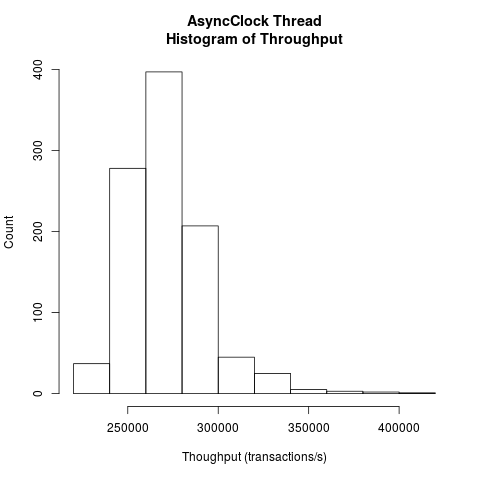
\includegraphics[height=.4\textheight]{async_thread_throughput_hist.png}
\caption{AsyncClock Thread Histogram of Throughput}
\label{async_thread_throughput}
\end{figure}

\begin{figure}[H]
\center
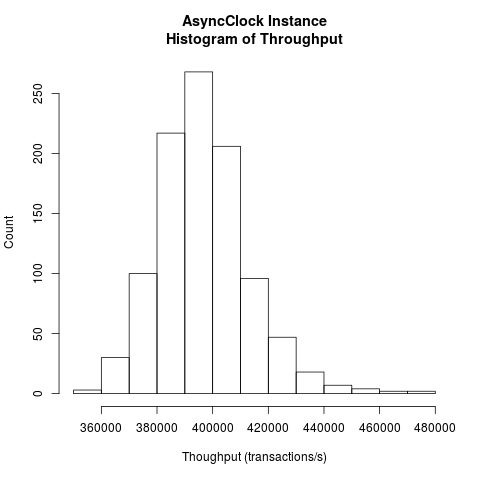
\includegraphics[height=.4\textheight]{async_instance_throughput_hist.png}
\caption{AsyncClock Instance Histogram of Throughput}
\label{async_instance_throughput}
\end{figure}

\begin{figure}[H]
\center
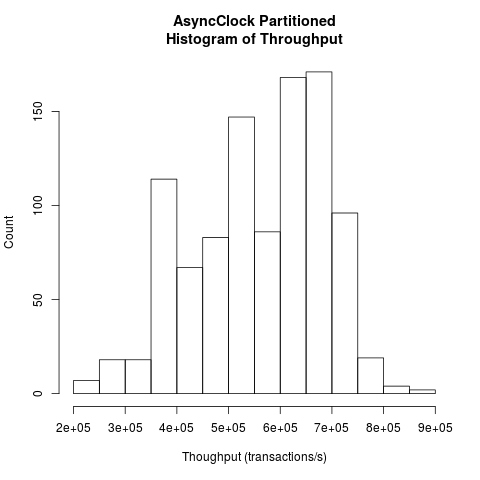
\includegraphics[height=.4\textheight]{async_partitioned_throughput_hist.png}
\caption{AsyncClock Partitioned Histogram of Throughput\label{async_partitioned_throughput}}
\end{figure}

\paragraph{AsyncClock results.}
Figures~\ref{async_thread_throughput}, \ref{async_instance_throughput}, and \ref{async_partitioned_throughput} show histograms of the throughput for the Thread, Instance, and Partitioned experiments, respectively.
The throughput for the Thread and Instance experiments appear to have ``regular'' distributions while the throughput for Partitioned is ``irregular.''
Transactions are randomly and statically allocated to execution threads in the Partitioned scheduler.
In the AsyncClock system, there are seven transactions where three correspond to Request, Response, and Tick, and the other four correspond to garbage collection actions for Client, Server, Counter, and System components.
Thus, there are $2^7 = 128$ mappings of transactions to execution threads.
Given the symmetry of threads, this results in 64 possible arrangements which are shown in Appendix~\ref{partition_tables} in Table~\ref{async_partitions}.
Some of these arrangements will place all transactions in one thread, leading to improved or degraded performance, e.g., `A'.
Some arrangements will place Request and Tick in different threads, allowing the potential concurrency among these actions to be exploited, e.g., `B'.
Some arrangements will place the Tick transaction and garbage collection action for Counter on different threads, creating lock contention, e.g., `C'.
Thus, the throughput for the Partitioned scheduler is a mixture of distributions corresponding to the different partitioning schemes.

\begin{figure}[H]
\center
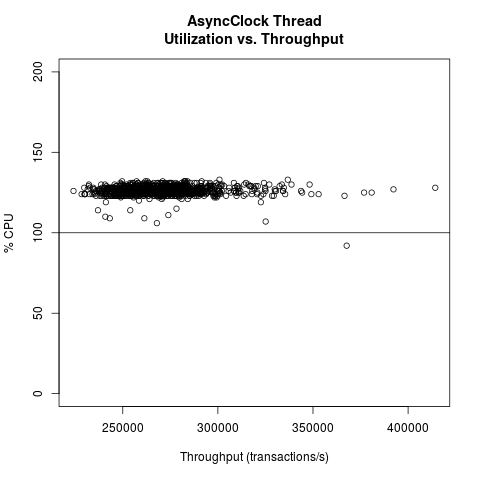
\includegraphics[height=.4\textheight]{async_thread_throughput_utilization.png}
\caption{AsyncClock Thread Utilization vs. Throughput}
\label{async_thread_throughput_utilization}
\end{figure}

\begin{figure}[H]
\center
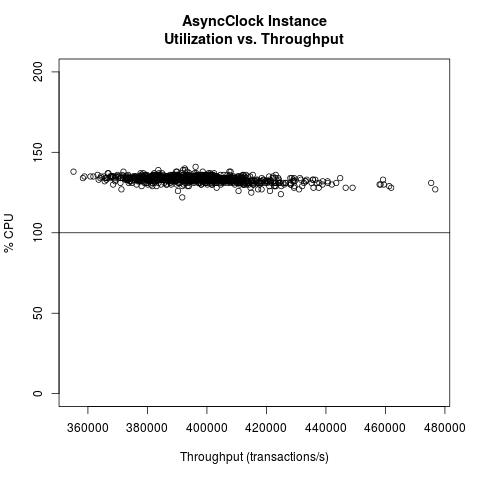
\includegraphics[height=.4\textheight]{async_instance_throughput_utilization.png}
\caption{AsyncClock Instance Utilization vs. Throughput}
\label{async_instance_throughput_utilization}
\end{figure}

\begin{figure}[H]
\center
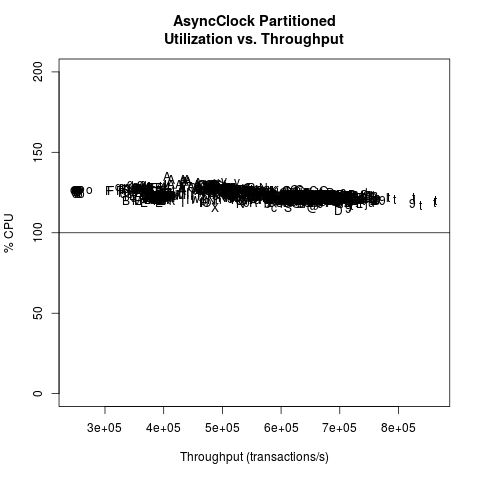
\includegraphics[height=.4\textheight]{async_partitioned_throughput_utilization.png}
\caption{AsyncClock Partitioned Utilization vs. Throughput}
\label{async_partitioned_throughput_utilization}
\end{figure}

Figures~\ref{async_thread_throughput_utilization}, \ref{async_instance_throughput_utilization}, and \ref{async_partitioned_throughput_utilization} show plots of utilization versus throughput for the Thread, Instance, and Partitioned experiments, respectively.
Most of the runs achieve a utilization greater than 100\%.
For the Instance and Partitioned schedulers, there appears to be slight trend where utilization decreases with increased throughput.
This is most likely the result of locking behavior where runs that (randomly) experience better locking behavior simultaneously achieve higher throughput and lower utilization due to less locking overhead.

\begin{figure}[H]
\center
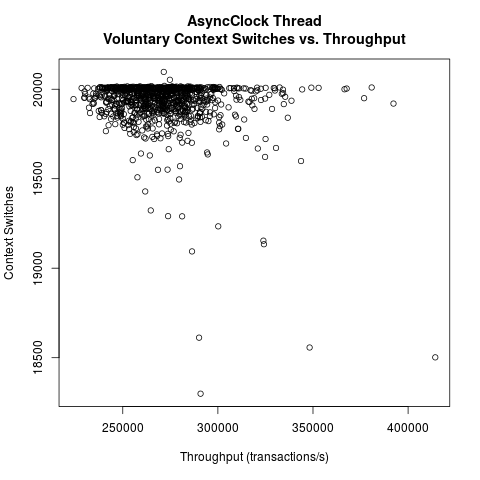
\includegraphics[height=.4\textheight]{async_thread_throughput_context.png}
\caption{AsyncClock Thread Voluntary Context Switches vs. Throughput}
\label{async_thread_throughput_context}
\end{figure}

\begin{figure}[H]
\center
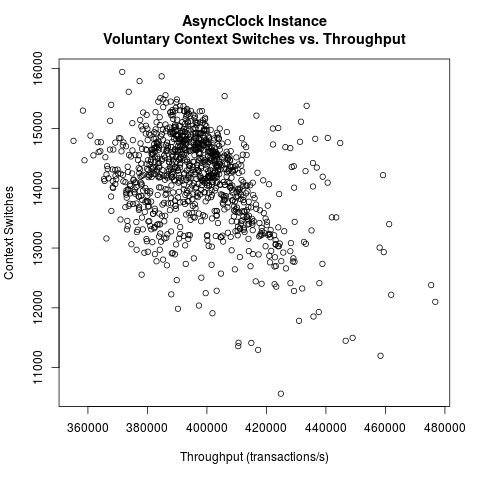
\includegraphics[height=.4\textheight]{async_instance_throughput_context.png}
\caption{AsyncClock Instance Voluntary Context Switches vs. Throughput}
\label{async_instance_throughput_context}
\end{figure}

\begin{figure}[H]
\center
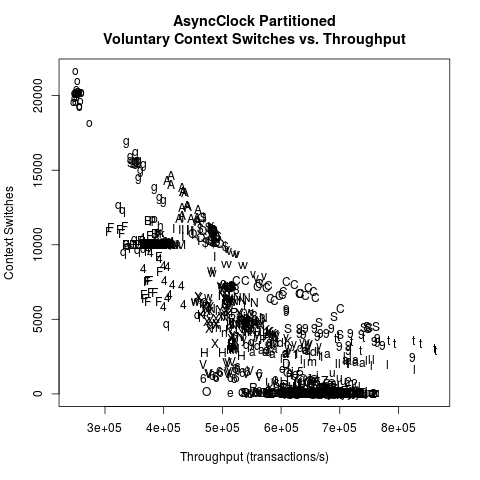
\includegraphics[height=.4\textheight]{async_partitioned_throughput_context.png}
\caption{AsyncClock Partitioned Voluntary Context Switches vs. Throughput}
\label{async_partitioned_throughput_context}
\end{figure}

Figures~\ref{async_thread_throughput_context}, \ref{async_instance_throughput_context}, and \ref{async_partitioned_throughput_context} show plots of voluntary context switches versus throughput for the Thread, Instance, and Partitioned experiments, respectively.
Voluntary context switches include the situation where a thread blocks while waiting for a lock and is swapped out.
The Thread scheduler appears to have a consistently high number of context switches.
This is expected since there are three threads competing for two processors.
The Instance scheduler has fewer context switches and perhaps shows a slight trend where throughput increases with fewer context switches.
As previously stated, this is most likely the result of locking behavior.
The Partitioned scheduler shows a strong trend of throughput increasing with fewer context switches.
Furthermore, the partitions appear to cluster together.
For example, all of the runs for partition `o' of Table~\ref{async_partitions} appear in the upper left of Figure~\ref{async_partitioned_throughput_context}, while the runs for partition `t' appear in the lower right.
In partition `o', thread 0 contains System, Counter, Tick, Request, and Response while thread 1 contains Server and Client.
This mapping serializes the execution (Request, Response, and Tick are on one thread) and is subject to contention arising from the Server and Client garbage collection actions competing with Request and Response.
In partition `t', thread 0 contains System, Counter and Tick while thread 1 contains Server, Client, Response, and Request.
The only contention in this mapping is between Response in thread 1 and Counter and Tick in thread 0.

\begin{figure}[H]
\center
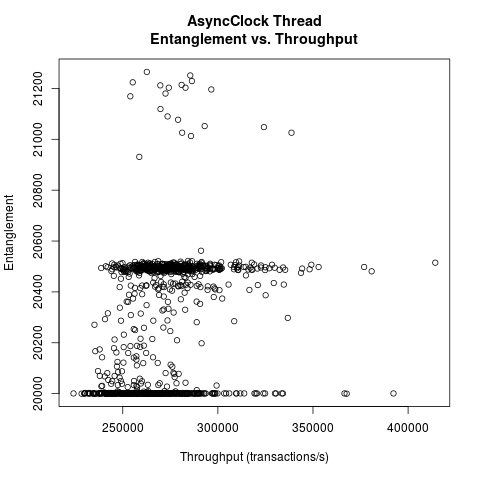
\includegraphics[height=.4\textheight]{async_thread_throughput_entanglement.png}
\caption{AsyncClock Thread Entanglement vs. Throughput}
\label{async_thread_throughput_entanglement}
\end{figure}

Figure~\ref{async_thread_throughput_entanglement} shows a plot of entanglement versus throughput for the Thread experiment.
The Thread scheduler has a minimum entanglement of 20,000, which is caused by the forced interleaving of the Request and Response threads, and a maximum entanglement of 30,000.
Thus, the lowest band in Figure ~\ref{async_thread_throughput_entanglement} corresponds to no entanglement with the Tick thread.
In these cases, the Linux thread scheduler executes the Request/Response threads first and the Tick thread second (or vice versa).
The generally low entanglement shows that the Linux scheduler prefers to serialize the execution.
This is reasonable given that the Thread scheduler is subject to a performance hit caused by context switches as previously described.
The upper band suggests a bound on the allowed entanglement.
One explanation for this behavior is that the Linux scheduler may limit context switches, which has the effect of limiting the entanglement in the Thread scheduler.
Another explanation is that the entanglement may be limited based on the threads starting at different times.

\begin{figure}[H]
\center
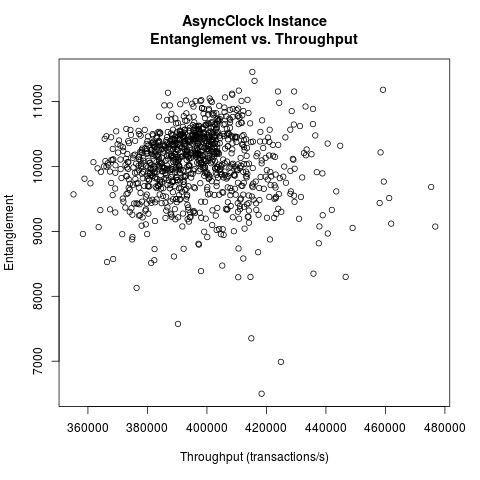
\includegraphics[height=.4\textheight]{async_instance_throughput_entanglement.png}
\caption{AsyncClock Instance Entanglement vs. Throughput}
\label{async_instance_throughput_entanglement}
\end{figure}

Figure~\ref{async_instance_throughput_entanglement} shows a plot of entanglement versus throughput for the Instance experiment.
The minimum entanglement is 0 and the maximum entanglement is 30,000\footnote{Let Transaction(Thread) indicate that the transaction was executed by the corresponding thread.  The following pattern when repeated 5,000 times generates an entanglement of 30,000:  Request(0) Tick(1) Response(0) Request(1) Tick (0) Response (1).}.
This plot does not appear to show a strong relationship between throughput and entanglement.

\begin{figure}[H]
\center
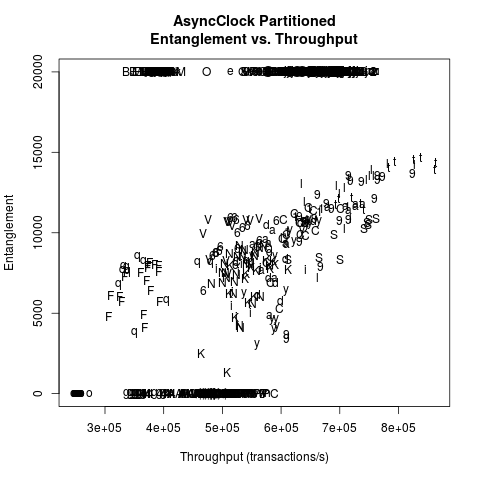
\includegraphics[height=.4\textheight]{async_partitioned_throughput_entanglement.png}
\caption{AsyncClock Partitioned Entanglement vs. Throughput}
\label{async_partitioned_throughput_entanglement}
\end{figure}

Figure~\ref{async_partitioned_throughput_entanglement} shows a plot of entanglement versus throughput for the Partitioned experiment.
This plot has a band at 20,000 that contains roughly half of the samples (513/1000).
These correspond to arrangements where Request and Response are mapped to different execution threads which forces an entanglement of 20,000.
Half of the remaining samples have no entanglement (246/1000).
These correspond to arrangements where the Request, Response, and Tick transactions are mapped to the same execution thread where no entanglement is possible.
The remaining quarter of the samples (241/1000) correspond to arrangements where Request and Response are in one execution thread while Tick is in the other.
These show varying degrees of entanglement with perhaps a slight trend toward increasing throughput with greater entanglement.
This is expected because the concurrency between Request and Tick can be exploited in these arrangements.

\begin{figure}[H]
\center
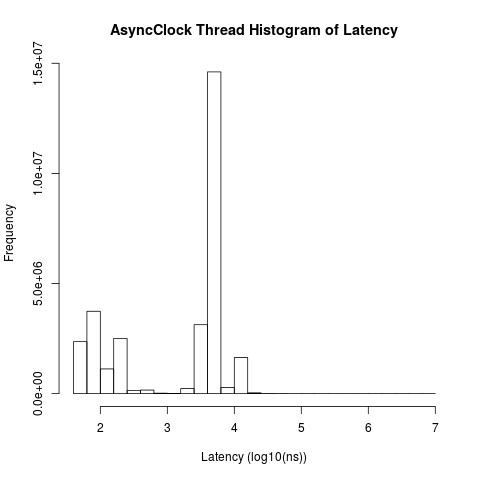
\includegraphics[height=.4\textheight]{async_thread_latency_hist.png}
\caption{AsyncClock Thread Histogram of Latency}
\label{async_thread_latency}
\end{figure}

\begin{figure}[H]
\center
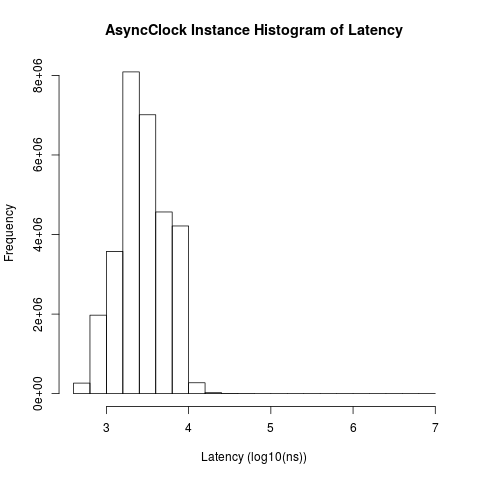
\includegraphics[height=.4\textheight]{async_instance_latency_hist.png}
\caption{AsyncClock Instance Histogram of Latency}
\label{async_instance_latency}
\end{figure}

\begin{figure}[H]
\center
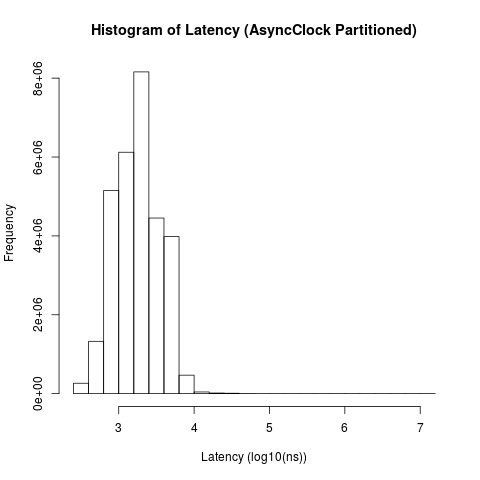
\includegraphics[height=.4\textheight]{async_partitioned_latency_hist.png}
\caption{AsyncClock Partitioned Histogram of Latency}
\label{async_partitioned_latency}
\end{figure}

Figures~\ref{async_thread_latency}, \ref{async_instance_latency}, and \ref{async_partitioned_latency} show histograms of the latency for the Thread, Instance, and Partitioned experiments, respectively.
All plots of latency use a logarithmic x-axis, as the latency distributions have very long tails.
For Thread, the mean latency of the transactions are as follows:
\begin{center}
\begin{tabular}{cr}
Tick     & 0.11769us \\
Request  & 5.30299us \\
Response & 5.63980us \\
\end{tabular}
\end{center}
Thus, the distribution on the left in Figure~\ref{async_thread_latency} corresponds to the latency of the Tick transaction while the distribution on the right corresponds to the latency of Request and Response.
In the Thread scheduler, Tick transactions can be executed in quick succession as they are in a tight loop.
For the Instance scheduler, the mean latency of the transactions are as follows:
\begin{center}
\begin{tabular}{cr}
Tick     & 5.22393us \\
Request  & 2.83083us \\
Response & 2.58799us \\
\end{tabular}
\end{center}
The Instance scheduler tends to serialize the execution of transactions for AsyncClock to avoid race conditions.
Thus, Tick has roughly twice the latency of Request and Response since Tick is always enabled while Request and Response are enabled by each other.
For Partitioned, the mean latency of the transactions are as follows:
\begin{center}
\begin{tabular}{cr}
Tick     & 2.49278us \\
Request  & 2.31450us \\
Response & 2.06478us \\
\end{tabular}
\end{center}
The work-conserving nature of the Partitioned scheduler allows it to achieve a lower average latency for all transactions when compared to the Instance scheduler.

\begin{figure}[H]
\center
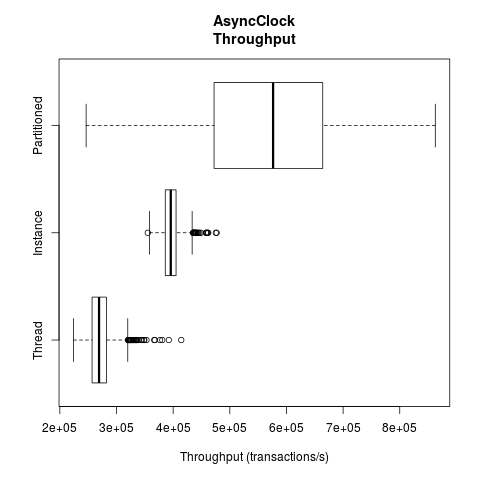
\includegraphics[height=.4\textheight]{async_throughput_box.png}
\caption{AsyncClock Throughput}
\label{async_throughput_box}
\end{figure}

Figure~\ref{async_throughput_box} shows a box plot of the throughput for the Thread, Instance, and Partitioned experiments.
The quantiles of the throughput in transactions/s for each scheduler are as follows:
\begin{center}
\begin{tabular}{crrrrr}
Scheduler   &       0\%   &    25\%     &    50\%     &    75\%     &   100\% \\
\hline
Partitioned &   246,370.0 &   472,679.2 &   576,411.0 &   664,042.5 &    862,717.0 \\
Instance    &   355,158.0 &   386,067.8 &   395,796.0 &   405,083.8 &    476,759.0 \\
Thread      &   224,107.0 &   256,876.0 &   269,193.5 &   282,329.0 &    414,293.0 \\
\end{tabular}
\end{center}
The work-conserving nature of the Partitioned scheduler allows it to achieve a higher throughput than the Instance scheduler, and its ability to avoid context switches allows it to achieve a higher throughput than the Thread scheduler.
However, the results also demonstrate the variability in the throughput due to the many modes of partitioning.
Thus, the Partitioned scheduler could be improved by using the race graph to avoid ``bad'' partitions.

\begin{figure}[H]
\center
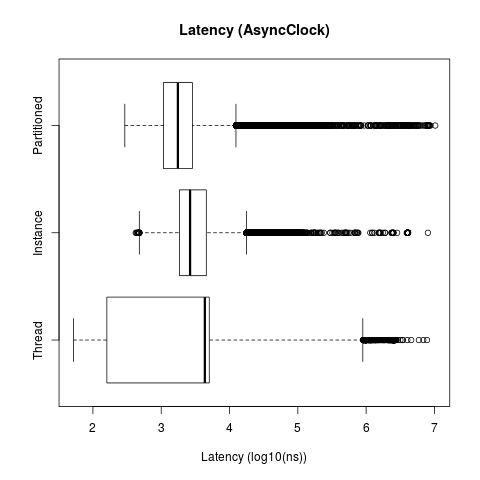
\includegraphics[height=.4\textheight]{async_latency_box.png}
\caption{AsyncClock Latency}
\label{async_latency_box}
\end{figure}

Figure~\ref{async_latency_box} shows a box plot of the latency for the Thread, Instance, and Partitioned experiments.
The quantiles of the latency (in ns) for each scheduler are as follows:
\begin{center}
\begin{tabular}{crrrrr}
Scheduler &       0\%  &    25\%  &    50\%  &    75\%  &   100\% \\
\hline
Partitioned & 293 & 1,075 & 1,754 & 2,861 & 10,296,400 \\
Instance    & 423 & 1,851 & 2,645 & 4,569 &  8,028,100 \\
Thread      &  52 &   160 & 4,352 & 5,051 &  7,791,400 \\
\end{tabular}
\end{center}
The Thread scheduler achieves the lowest latency via the Tick transaction due to its work-conserving nature and optimized locking scheme.

Both the Instance and Partitioned schedulers contain transactions for performing garbage collection.
These transactions do not actually perform any work since none of the transactions in the AsyncClock system allocate memory.
The Instance scheduler executed an average of 33,053 garbage collection actions per run while the Partitioned scheduler executed an average of 97,078 garbage collection actions per run.
The excessive number of collections performed by the Partitioned scheduler shows a potential problem between the garbage-collection-as-an-action idea and work conserving schedulers, as a work conserving scheduler can always find more work to do in garbage collection attempts.
Ideally, a scheduler would be designed to not even select a garbage collection action until it has a high probability of actually collecting garbage.

\clearpage

\begin{figure}[H]
\center
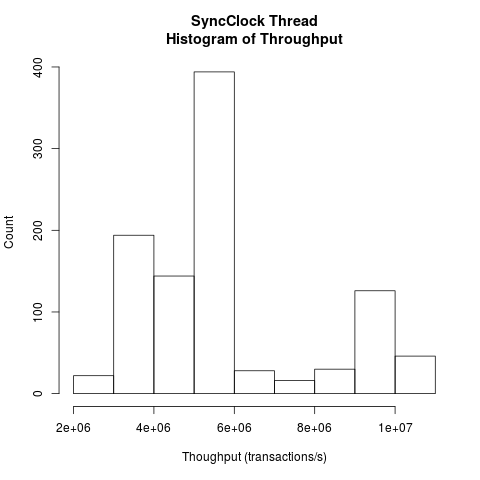
\includegraphics[height=.4\textheight]{sync_thread_throughput_hist.png}
\caption{SyncClock Thread Histogram of Throughput}
\label{sync_thread_throughput}
\end{figure}

\begin{figure}[H]
\center
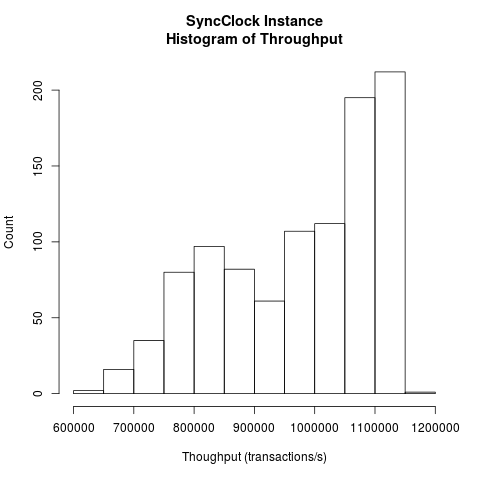
\includegraphics[height=.4\textheight]{sync_instance_throughput_hist.png}
\caption{SyncClock Instance Histogram of Throughput}
\label{sync_instance_throughput}
\end{figure}

\begin{figure}[H]
\center
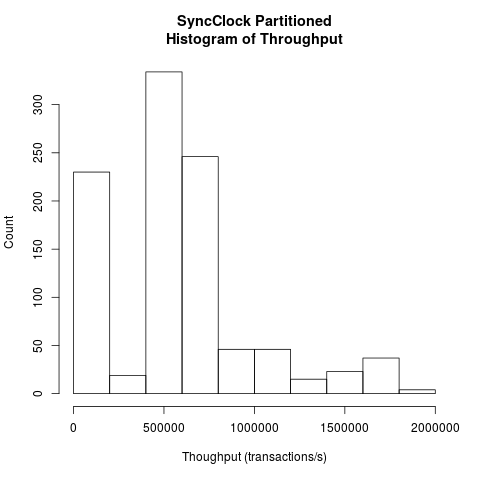
\includegraphics[height=.4\textheight]{sync_partitioned_throughput_hist.png}
\caption{SyncClock Partitioned Histogram of Throughput}
\label{sync_partitioned_throughput}
\end{figure}

\paragraph{SyncClock results.}
Figures~\ref{sync_thread_throughput}, \ref{sync_instance_throughput}, and \ref{sync_partitioned_throughput} show histograms of the throughput for Thread, Instance, and Partitioned experiments, respectively.
The throughput curves of the Thread and Instance experiments appear to be combinations of two or three distributions.
As in the AsyncClock experiments, the throughput for the Partitioned scheduler is a mixture of distributions arising from different partitioning schemes.
In the SyncClock system, there are two components and two transactions resulting in 8 possible partitions.
The list of partitions is given in Appendix~\ref{partition_tables} in Table~\ref{sync_partitions}.

\begin{figure}[H]
\center
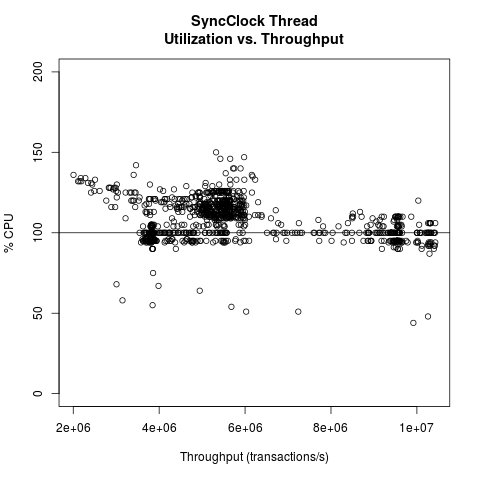
\includegraphics[height=.4\textheight]{sync_thread_throughput_utilization.png}
\caption{SyncClock Thread Utilization vs. Throughput}
\label{sync_thread_throughput_utilization}
\end{figure}

\begin{figure}[H]
\center
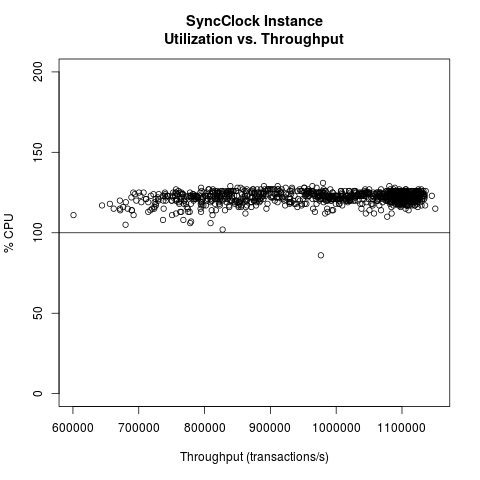
\includegraphics[height=.4\textheight]{sync_instance_throughput_utilization.png}
\caption{SyncClock Instance Utilization vs. Throughput}
\label{sync_instance_throughput_utilization}
\end{figure}

\begin{figure}[H]
\center
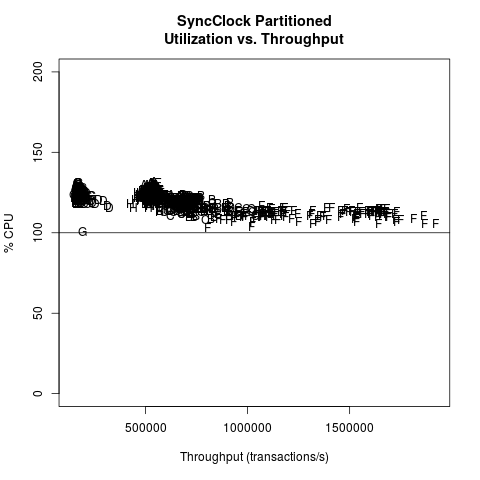
\includegraphics[height=.4\textheight]{sync_partitioned_throughput_utilization.png}
\caption{SyncClock Partitioned Utilization vs. Throughput}
\label{sync_partitioned_throughput_utilization}
\end{figure}

Figures~\ref{sync_thread_throughput_utilization}, \ref{sync_instance_throughput_utilization}, and \ref{sync_partitioned_throughput_utilization} show plots of utilization versus throughput for the Thread, Instance, and Partitioned experiments, respectively.
The utilization for the Thread scheduler decreases with increasing throughput.
This suggests that the Linux scheduler is serializing the execution of the threads which decreases utilization while avoiding lock contention which results in increased throughput.
Most of the runs for the Instance scheduler and Partitioned scheduler achieve a utilization greater than 100\% while a number of runs for the Thread scheduler do not.
The Instance scheduler shows a weak trend of increased utilization with throughput while the Partitioned scheduler shows a trend of decreased utilization with throughput.

\begin{figure}[H]
\center
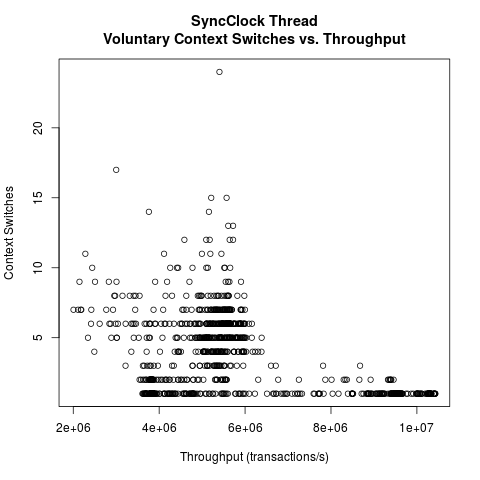
\includegraphics[height=.4\textheight]{sync_thread_throughput_context.png}
\caption{SyncClock Thread Voluntary Context Switches vs. Throughput}
\label{sync_thread_throughput_context}
\end{figure}

\begin{figure}[H]
\center
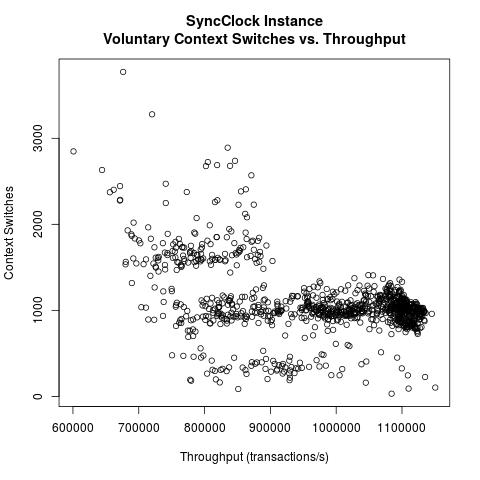
\includegraphics[height=.4\textheight]{sync_instance_throughput_context.png}
\caption{SyncClock Instance Voluntary Context Switches vs. Throughput}
\label{sync_instance_throughput_context}
\end{figure}

\begin{figure}[H]
\center
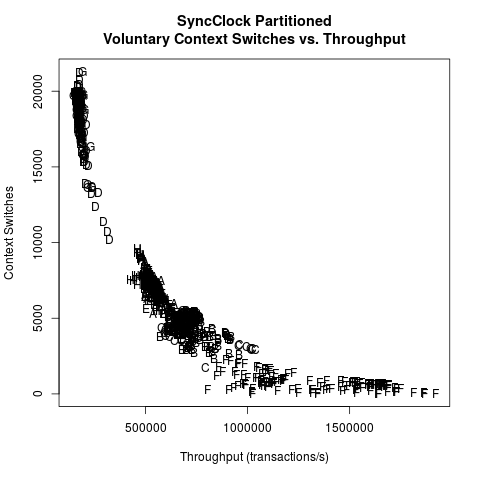
\includegraphics[height=.4\textheight]{sync_partitioned_throughput_context.png}
\caption{SyncClock Partitioned Voluntary Context Switches vs. Throughput}
\label{sync_partitioned_throughput_context}
\end{figure}

Figures~\ref{sync_thread_throughput_context}, \ref{sync_instance_throughput_context}, and \ref{sync_partitioned_throughput_context} show plots of voluntary context switches versus throughput for the Thread, Instance, and Partitioned experiments, respectively.
All show a trend where throughput increases with decreasing context switches.
Both the Thread and Instance experiments have a threshold where high throughput appears to require minimizing the number of context switches.
The plot for the Partitioned scheduler clearly shows an inverse relationship between throughput and context switches.

\begin{figure}[H]
\center
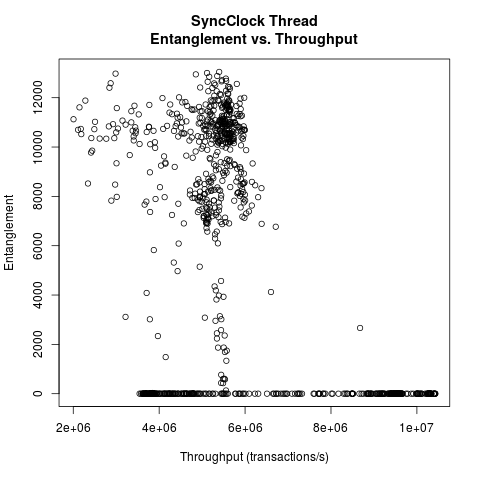
\includegraphics[height=.4\textheight]{sync_thread_throughput_entanglement.png}
\caption{SyncClock Thread Entanglement vs. Throughput}
\label{sync_thread_throughput_entanglement}
\end{figure}

\begin{figure}[H]
\center
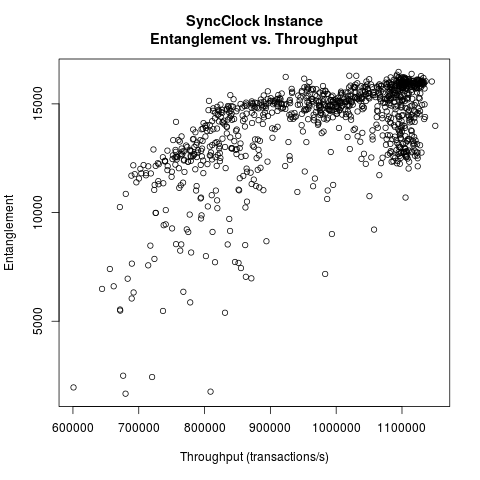
\includegraphics[height=.4\textheight]{sync_instance_throughput_entanglement.png}
\caption{SyncClock Instance Entanglement vs. Throughput}
\label{sync_instance_throughput_entanglement}
\end{figure}

\begin{figure}[H]
\center
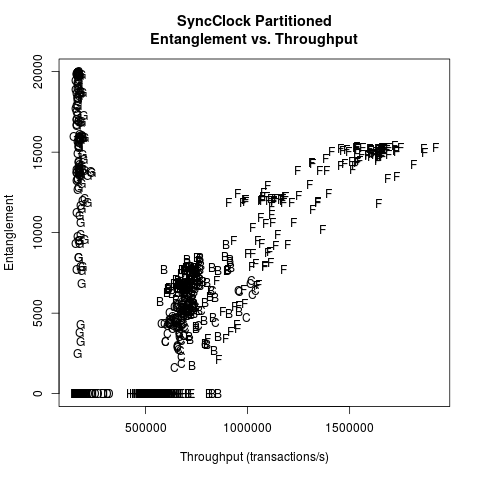
\includegraphics[height=.4\textheight]{sync_partitioned_throughput_entanglement.png}
\caption{SyncClock Partitioned Entanglement vs. Throughput}
\label{sync_partitioned_throughput_entanglement}
\end{figure}

Figures~\ref{sync_thread_throughput_entanglement}, \ref{sync_instance_throughput_entanglement}, and \ref{sync_partitioned_throughput_entanglement} show plots of entanglement versus throughput for the Thread, Instance, and Partitioned experiments, respectively.
The maximum entanglement for SyncClock is 20,000.
The plot of entanglement for the Thread scheduler resembles the plots of utilization and context switches.
The samples appear to be divided between concurrent (high entanglement, high context switch) and serial executions (low entanglement, low context switch).
For this system, it seems that it is more efficient to serialize the execution of the threads than to execute the threads concurrently and suffer context switches.

The plot of entanglement for the Instance scheduler shows a different trend where throughput increases with entanglement.
Thus, the Instance scheduler achieves high throughput when execution alternates between the threads.
The entanglement for the Partitioned scheduler appears to be a combination of three distributions.
The vertical line on the left consists of samples from the `G' partition which has maximal inter-thread conflicts and minimal opportunities for concurrent execution.
The horizontal line on the bottom (no entanglement) consists of samples from the `A', `D', `E', and `H' partitions which map Tick and Request to the same thread.
The execution is serialized with varying degrees of interference from the garbage collection actions.
The other samples contain the `B', `C', and `F' partitions which appear to show increasing throughput with entanglement.
The `F' partition has minimal inter-thread conflicts with maximal opportunities for concurrent execution.

\begin{figure}[H]
\center
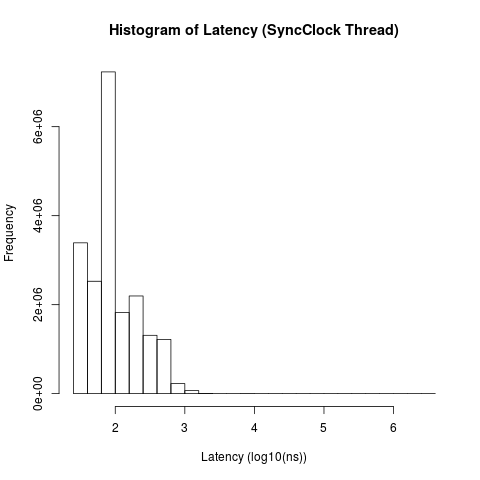
\includegraphics[height=.4\textheight]{sync_thread_latency_hist.png}
\caption{SyncClock Thread Histogram of Latency}
\label{sync_thread_latency}
\end{figure}

\begin{figure}[H]
\center
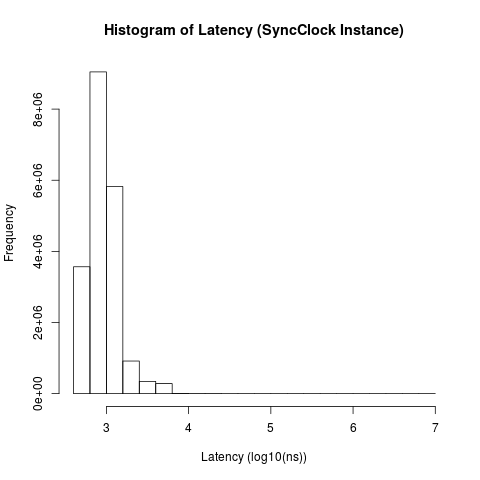
\includegraphics[height=.4\textheight]{sync_instance_latency_hist.png}
\caption{SyncClock Instance Histogram of Latency}
\label{sync_instance_latency}
\end{figure}

\begin{figure}[H]
\center
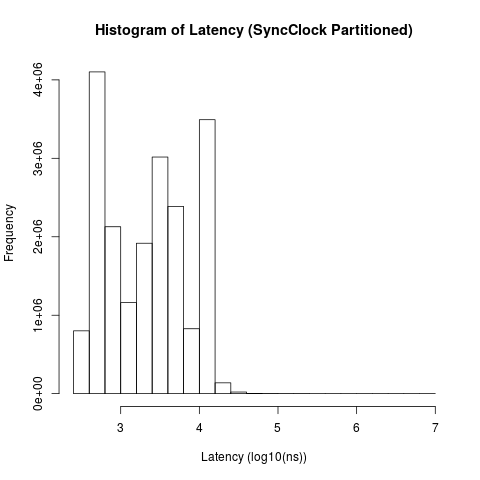
\includegraphics[height=.4\textheight]{sync_partitioned_latency_hist.png}
\caption{SyncClock Partitioned Histogram of Latency}
\label{sync_partitioned_latency}
\end{figure}

Figures~\ref{sync_thread_latency}, \ref{sync_instance_latency}, and \ref{sync_partitioned_latency} show histograms of the latency for the Thread, Instance, and Partitioned experiments, respectively.
All plots of latency use a logarithmic x-axis, as the latency distributions have very long tails.
For the Thread scheduler, the mean latency of the transactions are as follows:
\begin{center}
\begin{tabular}{cr}
Request &  72.952ns \\
Tick    & 207.145ns \\
\end{tabular}
\end{center}
The Request action does nothing more than acquire and release a lock which may explain its reduced latency.
For the Instance scheduler, the mean latency of the transactions are as follows:
\begin{center}
\begin{tabular}{cr}
Request & 1,085.32ns \\
Tick    & 1,070.57ns \\
\end{tabular}
\end{center}
For the Partitioned scheduler, the mean latency of the transactions are as follows:
\begin{center}
\begin{tabular}{cr}
Request & 4,117.71ns \\
Tick    & 4,069.06ns \\
\end{tabular}
\end{center}

\begin{figure}[H]
\center
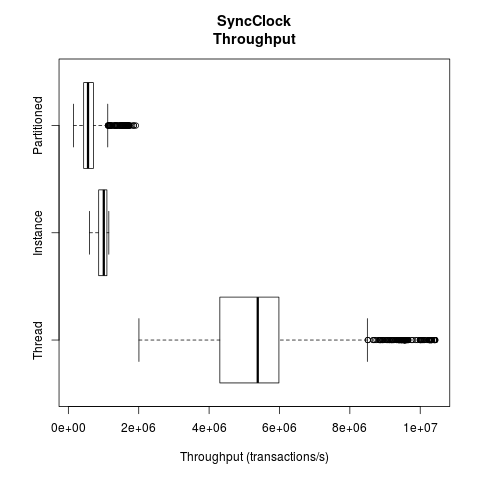
\includegraphics[height=.4\textheight]{sync_throughput_box.png}
\caption{SyncClock Throughput}
\label{sync_throughput_box}
\end{figure}

Figure~\ref{sync_throughput_box} shows a box plot of the throughput for the Thread, Instance, and Partitioned experiments.
The quantiles of the throughput in transactions/s for each scheduler are as follows:
\begin{center}
\begin{tabular}{crrrrr}
Scheduler   &       0\%   &    25\%     &    50\%     &    75\%     &   100\% \\
\hline
Partitioned &   146,788.0 &   439,051.0 &   558,954.5 &   711,073.8 &  1,919,680.0 \\
Instance    &   600,871.0 &   862,315.8 & 1,007,265.0 & 1,095,980.0 &  1,150,600.0 \\
Thread      & 2,005,940.0 & 4,308,048.0 & 5,382,440.0 & 5,983,532.0 & 10,428,200.0 \\
\end{tabular}
\end{center}
The Thread scheduler is clearly the best in terms of throughput.
The better performing partitions of the Partitioned scheduler are able to achieve the low end performance of the Thread scheduler.
In aggregate, however, the Instance scheduler appears to be better than the Partitioned scheduler.

\begin{figure}[H]
\center
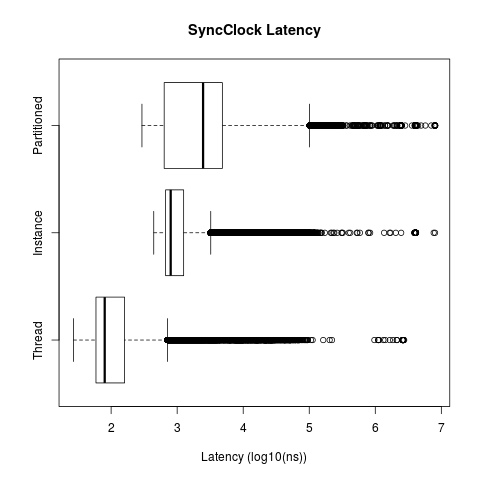
\includegraphics[height=.4\textheight]{sync_latency_box.png}
\caption{SyncClock Latency}
\label{sync_latency_box}
\end{figure}

Figure~\ref{sync_latency_box} shows a box plot of the latency for the Thread, Instance, and Partitioned experiments.
The quantiles of the latency (in ns) for each scheduler are as follows:
\begin{center}
\begin{tabular}{crrrrr}
Scheduler &       0\%  &    25\%  &    50\%  &    75\%  &   100\% \\
\hline
Partitioned & 293 &   636 & 2,469 & 4,835 &  8,100,990 \\
Instance    & 442 &   668 &   798 & 1,254 &  8,029,550 \\
Thread      &  27 &    59 &    80 &   160 &  2,736,960 \\
\end{tabular}
\end{center}
The Thread scheduler has the best latency by an order of magnitude.
This is unsurprising given the efficiency of the Thread implementation.

\section{Summary}

Perhaps the most interesting part of the implementation of the \rcgo{} run-time system is the scheduler.
Fairness, safety, and responsibility are identified as the three essential requirements for any scheduler and we illustrate how these may be accomplished in a variety of designs.
Two multi-threaded schedulers were implemented.
The Instance scheduler is based on a shared work queue of instances while the Partitioned scheduler is based on partitioning transactions among different scheduler threads.
We used throughput, latency, and utilization as metrics for evaluating schedulers for reactive components and collected data for the Instance and Partitioned schedulers by executing the AsyncClock and SyncClock systems.
The reactive component schedulers were then compared to custom implementations of the same systems using the pthreads library.
%% The results show that the reactive component schedulers are viable as event schedulers but will require improvement to become competitive with threads.
%% Moving from interpretation to compilation, reducing locking overhead, and reducing the overhead of precondition evaluation seem to be promising areas for improvement.

The AsyncClock and SyncClock experiments demonstrate both the viability of reactive components as an event system and that more work is necessary to improve the design and implementation of the run-time system.
The motivation for events was to facilitate (logical) concurrency while avoiding the overhead of context switching associated with assigning each task to a thread.
The performance of the Partitioned scheduler over the Thread implementation of AsyncClock demonstrates this idea.
As was previously mentioned, events can be combined with multi-threading but care must be taken to ensure proper synchronization.
In the reactive component model, the burden of correct synchronization is placed on the scheduler instead of the developer.

The AsyncClock system is illustrative in that it shows the advantage of events over threads but is nevertheless unrealistic as it intentionally overloads the system.
The SyncClock system represents a scenario in which there are adequate resources for each thread.
In this situation, the Instance and Partitioned schedulers perform an order of magnitude worse than the Thread implementation.
This prompts the question:  can reactive components be as efficient as threads?
While we cannot answer this question definitively, the act of converting a reactive component program to a threaded program does provide evidence that it may be possible to make reactive components as efficient as threads.
The procedure for converting a reactive component program to a threaded program involves 1) creating a reader/writer lock for each component instance, 2) creating a thread for each transaction, 3) creating a condition variable and mutex for each precondition, 4) creating a critical section for each transaction, and 5) signaling affected transactions after the critical section.
It seems feasible that this procedure can be automated.
Thus, a system of reactive components can be converted to threads or scheduled as events depending on the resources available and nature of the transactions in the system, but doing so is left for future work.

%% \section{Scheduler}

%% \paragraph{Fairness.}
%% The only requirement for a scheduler for reactive components is fairness.
%% Fairness, as applied to reactive components, means that every action receives an infinite number of opportunities to execute.

%% \paragraph{Single-threaded and multi-threaded designs.}
%% A fair single-threaded scheduler is straight-forward to implement by cycling through all the actions in a round-robin fashion.
%% Minimizing scheduling overhead by not giving opportunities to disable actions is the main optimization.
%% The same principles apply to multi-threaded schedulers with added challenge of avoiding data races.
%% That is, a multi-threaded scheduler cannot simultaneous execute two actions that may mutate the same state.
%% A multi-threaded scheduler must either prevent the various threads from selecting conflicting actions or implement a protocol that allows the threads to negotiate the conflict.
%% A scheduler might prevent conflicts by computing a schedule for each thread with explicit synchronization points.
%% The advantage of this approach is that fairness is easily enforced.
%% The drawbacks of this approach is that it is very rigid and may lead to excessive overhead and idle time waiting for synchronization.
%% Conflict can be negotiated by either selecting a different action (deferral) or blocking until there is no longer a conflict.
%% To enforce fairness, an action cannot be deferred indefinitely.
%% The remainder of the discussion focuses on the design and implementation of a multi-threaded scheduler.

%% \paragraph{Steady-state assumption.}
%% To make the design of the system tractable, we assume that the system achieves a steady-state for all executions.
%% For infinite executions, this typically involves the use of flow control/feedback to prevent producers of work from overrunning consumers of work.
%% For finite executions, the system must always achieve a \emph{fixed-point} which is a state where every action is disabled.
%% Suppose a producer task P executes on one thread and produces one work item for a consumer task C executing on another thread.
%% Furthermore, suppose that P is always enabled and is executed proportionally faster than C.
%% An infinite execution is fair, i.e., it will have and infinite number of P's and C's, however, C will never ``catch up'' to P.
%% If memory is allocated for every item produced by P, then the system will require an unbounded amount of memory.
%% In general, if a producer task that generates $n$ work items for a consumer task, then the consumer task must be executed $n$ times faster to ``keep up.''
%% The steady-state assumption means that the relative frequency of action executions is irrelevant for correctness.
%% We believe the assumption of a steady-state is not overly restrictive as all real-world systems have this property.

%% \paragraph{Motivation for a partitioned scheduler.}
%% A straightforward approach to constructing a multi-threaded scheduler is to place all actions on a global list and have each thread execute the next action on the list.
%% This organization has three potential problems.
%% First, the global list is a shared resource.
%% As the number of processors increases, so will contention on the list.
%% Second, locking is mandatory to avoid data races.
%% To execute an action, a thread must acquire a lock for all instances involved in the action.
%% Third, this approach requires extra logic for good cache behavior.
%% A thread may not want the next action on the list if the action has no affinity for the thread.

%% In a partitioned scheduler, the actions are partitioned among the available threads.
%% This organization eliminates contention over a shared global list and has the potential for good cache behavior.
%% Data races can be avoided through partitioning and locking.
